\newpage
\section{Deep Learning Architecture}

\begin{itemize}
  \item TCN Design so causal conv, conv1d, activation functions etc.
  \item Learning - Loss Functions, Explain problem of overfitting and why we need regularisation, optimisers (explain gradient descent), learning rate
\end{itemize}

\subsection{Aims of the Deep Learning Model}
Referring back to \hyperref[sec:problem]{section 1.2}, the overall problem 
is to implement a model that can output gyroscopic corrections 
$\Delta\boldsymbol{\omega}_t = [\Delta\omega_x,\Delta\omega_y,\Delta\omega_z]^\top$
that when subtracted from our measured angular rate, and fused with other
sensors such as an accelerometer and magnetometer leads to an orientation 
estimate, that is more accurate to the ground truth orientation of an 
object compared with only sensor fusion. 

The motivation for learning $\Delta\boldsymbol{\omega}_t$ 
comes from the fact that while sensor fusion techniques of downweighting 
or skipping of the accelerometer and magnetometer when they are unreliable
, drift cannot be mitigated due to the accumulation of gyroscopic bias 
and noise \fixme{cite, cite2}. 

\subsection{Model Selection}
\subsubsection{Recurrent Neural Networks (RNNs)}
The first type of model that was considered is a RNN. RNNs stem from an 
idea of recurrence, that is that the output depends on some input at time
t and an internal state of the model that holds information about previous
outputs of the model. The general idea can be described by the equation

\begin{equation}
\hat{y} = f_{model}(x_t, h_{t-1})
\end{equation}

where $\hat{y}$ is the output, $f_{model}$, is a function that describes the model,
$x_t$ is the input at time t, and $h_{t-1}$ is a vector state that
describes the internal state of the model at the previous time step. Expanding
on this the state of the model is updated as follows

\begin{equation}
h_t = f_w(x_t, h_{t-1})
\end{equation}

where $f_w$ is a function with weights $w$. This expands to the equations

\begin{equation}
\hat{y} = W_{hy}^T h_t
\end{equation}

\begin{equation}
h_t = \phi(W_{hh}^T h_{t-1} + W_{xh}^T x_t)
\end{equation}

where $W_{hh}^T, W_{hy}^T, W_{xh}^T$ are a set of weight matrices that are
reused for every time step, and $\phi$ represents an arbitrary activation function.


\begin{figure}[htp]
    \centering
    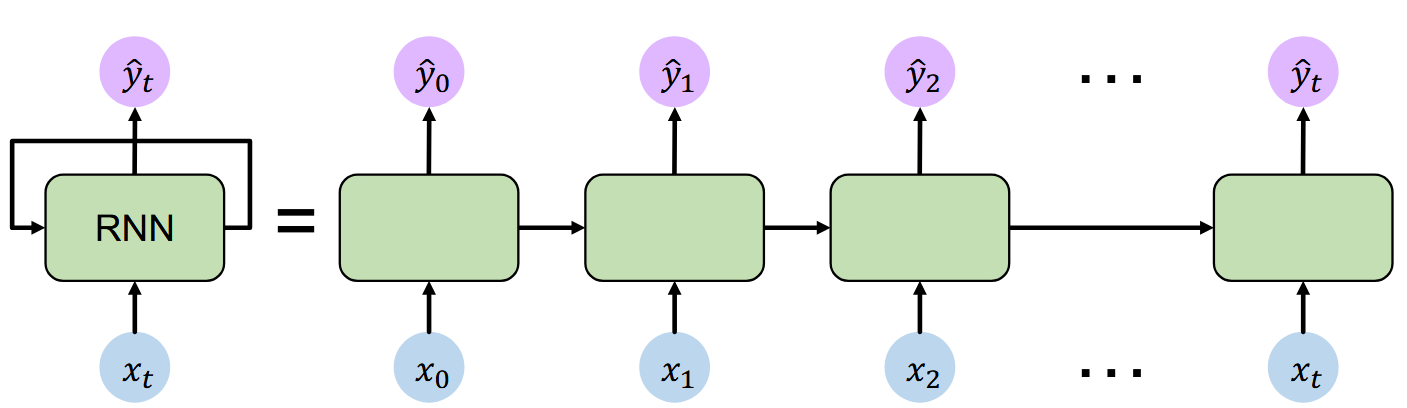
\includegraphics[width=10cm]{./figures/Model/RNN.png}
    \caption{RNN structure \fixme{cite3}}
    \label{fig:RNN}
\end{figure}

\hyperref[fig:RNN]{Figure 3} shows the unrolled flow of the RNN, where the arrows between each
block represents the passing of $h_t$, from one input to the next. The point
of the recurrence state $h_t$, is to show how the output of the model depends
on context from previous inputs plus $h_t$. This is especially relevant in our case, as
described in \hyperref[sec:gyroint]{section 3.1.1}, the accumulation of 
gyroscopic errors comes from the integration of the angular rate. As these
errors accumulate, the current error depends on the history of the gyroscope 
measurements. 

There are many problems with RNNs however, the biggest being the problem of exploding/vanishing
gradients. RNNs are trained via backpropagation through time, which propagates gradients across
timesteps. For long sequences, computing the gradient with respect to $h_0$ involes many factors
of repeated multiplication of Jacobians across time. This can lead to many values of the computation
being greater than 1, which explodes gradients leading to unstable training.
In the case, where many values are less than 1, this causes vanishing gradients where learning long-range
dependencies becomes difficult. Additionally, as the hidden state $h_t$ is propagated sequentially through
time, when performing backpropagation, training cannot be parallelised over timesteps. This results in 
a high training times compared to convolutional models.

Updated versions of the RNN have been proposed to solve the problem of vanishing and exploding
gradients. These being Long Short Term Memory (LSTM) and Gated Recurrent Units (GRUs). These methods
exploit the use of a cell state that does not need to do perform repeated multiplication of Jacobians,
however they are still subject to long training times \fixme{cite} and the gradient problem is not fully 
solved but mitigated \fixme{cite, cite}.

\subsubsection{Convolutional Neural Networks (CNNs)}
The next type of model considered was the CNN, even though typically it is used in computer
vision tasks; it has seen wide use in research relating to drift reduction \fixme{cite, cite, cite}. 
This model is based on the idea of convolving input data with a learnable filter to extract local 
features in the input data. The filter can be thought of like a window that slides over the 
data, and each filter has a defined set of weights in which it multiplies with input data.
This convolution operation can be described by the equation below: 

\begin{equation}
  z_f[t] = b_f + \sum_{c=1}^{C_{in}} \sum_{k=0}^{K-1} w_{f,c}[k] x_c[t+k- \lfloor K/2 \rfloor]
\end{equation}
\label{eq:12}

\begin{equation}
  y_f[t] = \phi(z_f[t])
\end{equation}

where $y_f[t]$, is the output of filter f, $b_f$ is a bias, $C_{in}$ is the input channels 
(for our case $C_{in}$ would be 3 for $\omega_x, \omega_y, \omega_z$), $K$ is the 
kernel/filter width, $w_{f,c}$ is the weights of the filter for a specific channel, 
$x_c$ is the input data of that channel, and $\phi$ is an arbitrary non-linear activation
function (typically ReLU).

For example if $K = 3$, the convolution will occur 
of the timesteps $x[t-1], x[t], x[t+1]$, this is how the convolution extracts local features 
in the input data.
 
Typically, these CNNs are made up of layers, where in each layer the number of filters 
grow e.g. $L1 = 16, L2 = 32, L3 = 64$ etc. These additional filters in later layers allow the
model to learn more complex feature sets based on the previous layers' filter. Zeiler et al.
\fixme{cite} shows this in their figure 2 where their convolutional network is used for image
classification.

\begin{figure}[H]
    \centering
    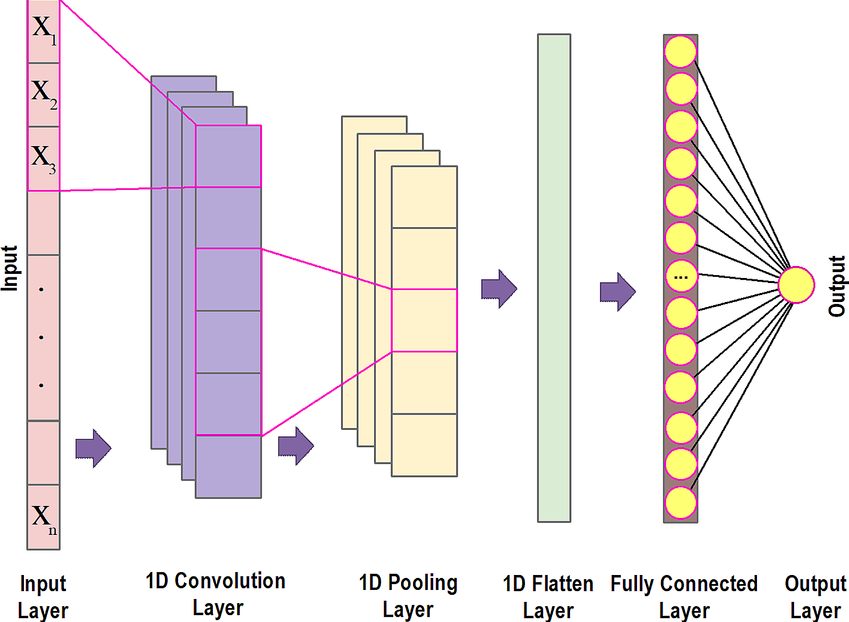
\includegraphics[width=10cm]{./figures/Model/CNN.png}
    \caption{1D CNN structure \fixme{cite}}
    \label{fig:CNN}
\end{figure}


CNNs are more attractive than RNNs due to its ability to be efficiently
trained by using parallelisation\fixme{cite}. As stated before, RNNs cannot exploit 
this, but CNNs can. This leads to the ability to test multiple different
iterations of a model where parameters and loss functions may be changed
to explore what effects they may have \fixme{see section}. CNNs also do
not suffer from vanishing//exploding gradients and are seen to be more
stable during training\fixme{cite}. 

However, unlike RNNs, baseline CNNs cannot produce outputs due to significant 
temporal information. It can extract local features and in 1D convolutions
it has some ability to traverse backwards through time but not to any
significant degree. As seen in \hyperref[sec:gyroint]{section 3.1.1}, 
the accumulation of drift is due to the integration of the angular rate
as we move forward in time. 

\subsubsection{Temporal Convolutional Networks (TCNs)}
TCNs are an extension of the baseline CNN and include two main differences
in their implementation as shown by Bai et al.\fixme{cite}. These differences
are the use of dilations that grow the receptive field allowing the network
to look back further in time and learn long-term information. Furthermore,
causal convolutions meaning, that the convolution operation cannot
look forward in time. To explain causality we can look back at  
\hyperref[eq:12]{equation 12} and modify this so 

\begin{equation}
  z_f[t] = b_f + \sum_{c=1}^{C_{in}} \sum_{k=0}^{K-1} w_{f,c}[k] x_c[t-k]
\end{equation}

\begin{equation}
  y_f[t] = \phi(z_f[t])
\end{equation}

The difference is that the $k$ is subtracted from $x[t]$. The causality
is enforced here as at time $t$, we cannot access future information unless
the model is to be used after data collection and not in a real time 
setting.

Dilations allow the model to look further back in time without the need
of increasing parameters for the same $K$ and $C_{in}$ used in convolutions. This is best represented in
the figure 5.

\begin{figure}[H]
    \centering
    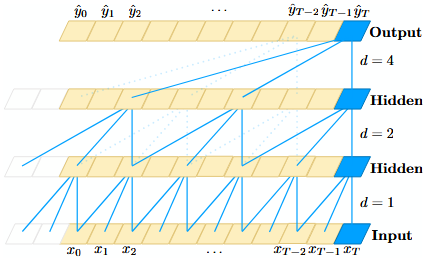
\includegraphics[width=10cm]{./figures/Model/dilations.png}
    \caption{CNN structure with dilations \fixme{cite}}
    \label{fig:dilations}
\end{figure}

As we can see in the diagram, as the dilations increase layer by layer
the output to the next layer looks further back into the history of
$x[t]$. This can be modelled by the equation

\begin{equation}
  z_f[t] = b_f + \sum_{c=1}^{C_{in}} \sum_{k=0}^{K-1} w_{f,c}[k] x_c[t-dk]
\end{equation}

where $d$ is the dilation factor of the layer. 


\subsubsection{Summary and Choice}
In summary, the choice has been to select the TCN. This is because it 
has the ability to look back in history and model long-term dependencies
between data, something baseline CNN cannot do. Additionally, like a CNN
it is quicker and more stable in training unlike an RNN. However, the TCN
does have its problems, these being extra data storage during its operation
and domain transfer. Unlike RNNs which only have store $h(t)$, TCNs needs
to take in a raw sequence upto its effective history length \fixme{cite}.
Domain transfer refers to transferring a model that has been trained in 
one domain (i.e. small receptive field) and applied to another domain
(i.e. large receptive field), where the TCN may perform poorly due to 
this change in domain.


\subsection{TCN Design and Parameters}
\subsection{Learning}
